\documentclass[a4j,12]{jarticle}
\usepackage{exp1}

%\pagestyle{empty}
%%%%%%%%%%%%%%%%%%%%%
%%%レポート作成者情報の入力
%%%班
\def\group{グループ番号}
%%%学籍番号
\def\idnumber{1315193T}
%%%氏名
\def\name{薛 宇航}
%%%実験月日月
\def\expmontho{月}
\def\expdayo{日}
%%%実験月日
\def\expmontht{月}
\def\expdayt{日}
%%%実験月日
\def\expmonthth{月}
\def\expdayth{日}
%%%レポート提出月日
\def\deadlinem{01}
\def\deadlined{19}
%%%共同実験者1
\def\groupmembero{1305194T 中山 峻一}
%%%共同実験者2 居なかった場合には{}だけにする.
\def\groupmembert{1385195T 藤原 巧}
%%%共同実験者3 居た場合には{}内に学籍番号と氏名を入力する.
\def\groupmemberh{1365196T 和田 佳大}
%%%%%%%%%%%%%%%%%%%


\begin{document}

\title{
\vspace{1cm}{\LARGE 平成27年度}\\
% \vspace{1em}
\begin{spacing}{1.5}
{\Huge ディジタル信号処理}\\
{\huge --ニューラルネットワークを用いた音の認識--}
\end{spacing}
\author{}
\date{}
}%%表紙の情報、、入力忘れないように
\maketitle
\vspace{5cm}
{\Large
\begin{spacing}{1.2}
%%%\noindent\hspace{20em}\underline{班:\group 班}\\
%%%\hspace{20em}\underline{実験日時:\expmontho 月\expdayo 日}\\
%%%\hspace{20em}\underline{    :\expmontht 月\expdayt 日}\\
%%%\hspace{20em}\underline{    :\expmonthth 月\expdayth 日}\\
\hspace{20em}\underline{レポート提出日:\deadlinem 月\deadlined 日}\\
\hspace{20em}\underline{学籍番号:\idnumber}\\
\hspace{20em}\underline{氏  名:\name}\\
\end{spacing}
}
\thispagestyle{empty}
\newpage
\setcounter{page}{1}      %ページ番号リセット


\section{課題内容}
あ〜おまでの5クラスの分類のデータがある。各ファイルの長さを3.5秒で統一して短時間フーリエ変換を計算し、特徴量抽出を行うこと。短時間分析区間は、24msecサンプル点、4msecシフトとして対数パワースペクトルを計算すること。\par
次に、学習データから得られた対数パワースペクトるを、全学習データを用いて平均ベクトルを計算する。この平均ベクトルを学習データの対数パワースペクトル、及びテストデータの対数パワースペクトルから減算して、ニューラルネットワークに入力する。
\section{レポート内容}
\subsection{レポート結果}
今回、課題は完全に終わったと言えません。なお、できるところまでだけレポートとしてまとめて提出する。\par
資料により、重みの更新式は以下の式(1)と式(2)のように一般化した:
\begin{eqnarray} 
  n\_w=^2_{kj}=w^2_{kj}+2(d_k[n]-g_k[n])*f'(u_k)*g_j\\
  n\_w=^1_{ji}=w^1_{jk}+{\sum_k(d_k-g_k)*f'(u_k)*w_{kj}}*f'(u_j)*x_i[n]
\end{eqnarray}%%数式
ここで、特にf(x)はシグモイド関数で、f'(x)はこの関数の微分で、それぞれ以下の式(3)、(4)のようになる。
\begin{eqnarray}
  f(x)=\frac{1}{1+e^{-x}}\\
  f'(x)=f(x)*(1-f(x))
\end{eqnarray}

以上より、20回繰り返し学習後、d[n]とy[n]の二乗誤差erをgnuplotで出力した結果は以下の図1のようになる。
\begin{figure}[htpb]
  \begin{center}
    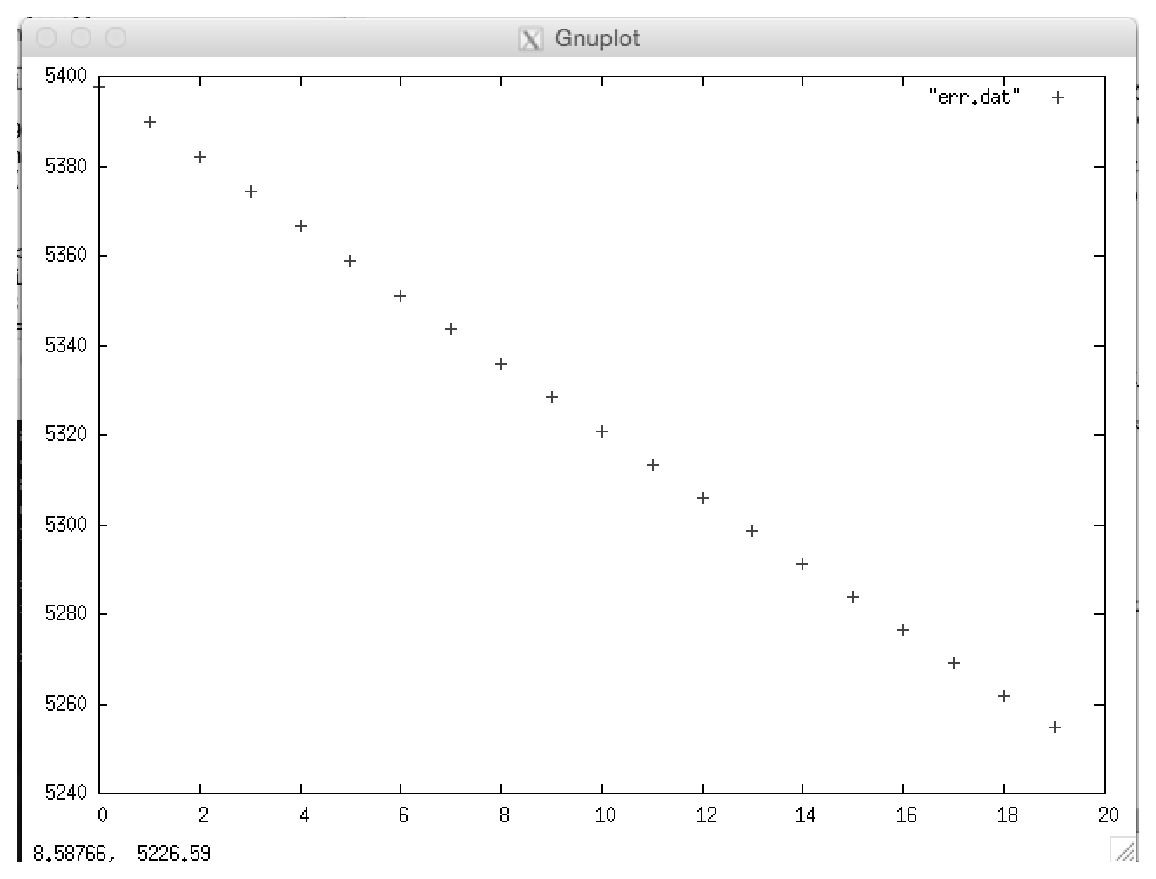
\includegraphics[width=15cm]{err.eps}
    \caption{学習回数と誤差の関係}
    \label{micon}
  \end{center}
\end{figure}
一応、誤差がどんどん減ることが確認できた。
\subsection{使用するプログラム}
今回は、計算速度をあげるため、ファイルをとりあえず二つに分けた。一つ目は、パワースペクトルまでは出した。もう一つ目は、このパワースペクトルを読み込んで、ニューラルネットワークに通す作業をする。
\begin{lstlisting}[caption=パワースペクトル計算するプログラム,label=ラベル]
#include <stdio.h>
#include <math.h>
#include <stdlib.h>
#include <time.h>

#define A 0
#define I 1
#define U 2
#define E 3
#define O 4
#define MAX_SIZE 28000
#define Pi 3.14159265358979

int main()
{
  char filename[5][128]={"a.raw","i.raw","u.raw","e.raw","o.raw"};

  int size,i,j,n,k,count;

  short **data;//ファイルデータ
  short ***data_data;//分割されたデータを保存する場所
  double ***real_data_data;
  double ***image_data_data;
  double ***F_data_data;
  FILE *file_input;
  FILE *file_output;
  
  double ***power;
  
  //dataは全部アイウエオで五種類
  if( (data=(short **)calloc(5,sizeof(short *))) == NULL ){
    fprintf(stderr,"cannot calloc memory **data.\n");    exit(-1);
  }
  //一種類のデータにはデータ数3.5*8000=28000個
  for(i=A;i<=O;i++){
    if( (data[i]=(short *)calloc(MAX_SIZE,sizeof(short))) == NULL ){
      fprintf(stderr,"cannot calloc memory *data%d.\n",i+1);    exit(-1);
    }
  }
  //とりあえずファイルを読み込む
  for(i=A;i<=O;i++){
    if((file_input=fopen(filename[i],"rb"))==NULL){
      fprintf(stderr,"cannot read %s. \n",filename[i]);exit(-1);
    }
    fread(data[i],sizeof(short),MAX_SIZE,file_input);//結果をdataに保存する
    fclose(file_input);
  }
  //分割データの保存先
  if((data_data=(short ***)calloc(5,sizeof(short **)))==NULL){
    fprintf(stderr,"cannot calloc ***data_data.\n");
  }
  //      フーリエ変換した実数部
  if((real_data_data=(double ***)calloc(5,sizeof(double **)))==NULL){
    fprintf(stderr,"cannot calloc ***real_data_data.\n");
  }
  //      フーリエ変換した虚数部
  if((image_data_data=(double ***)calloc(5,sizeof(double **)))==NULL){
    fprintf(stderr,"cannot calloc ***image_data_data.\n");
  }
  //      フーリエ変換した結果
  if((F_data_data=(double ***)calloc(5,sizeof(double **)))==NULL){
    fprintf(stderr,"cannot calloc ***F_data_data.\n");
  }
  //      パワースペクトルの自然対数を保存する
  if((power=(double ***)calloc(5,sizeof(double **)))==NULL){
    fprintf(stderr,"cannot calloc ***power.\n");
  }
  for(i=A;i<=O;i++){
    size=(MAX_SIZE-(192-32))/32;
    if((data_data[i]=(short **)calloc(size,sizeof(short *)))==NULL){
      fprintf(stderr,"cannot calloc **data_data[%d]\n",i+1);exit(-1);
    }
    if((real_data_data[i]=(double **)calloc(size,sizeof(double *)))==NULL){
      fprintf(stderr,"cannot calloc **real_data_data[%d]\n",i+1);exit(-1);
    }
    if((image_data_data[i]=(double **)calloc(size,sizeof(double *)))==NULL){
      fprintf(stderr,"cannot calloc **image_data_data[%d]\n",i+1);exit(-1);
    }
    if((F_data_data[i]=(double **)calloc(size,sizeof(double *)))==NULL){
      fprintf(stderr,"cannot calloc **F_data_data[%d]\n",i+1);exit(-1);
    }
    if((power[i]=(double **)calloc(size,sizeof(double *)))==NULL){
      fprintf(stderr,"cannot calloc **power[%d]\n",i+1);exit(-1);
    }
    
    for(j=0;j<size;j++){
      if((data_data[i][j]=(short *)calloc(192,sizeof(short)))==NULL){
	fprintf(stderr,"cannot calloc *data_data[%d][%d]\n",i+1,j+1);exit(-1);
      }
      if((real_data_data[i][j]=(double *)calloc(192,sizeof(double)))==NULL){
	fprintf(stderr,"cannot calloc *real_data_data[%d][%d]\n",i+1,j+1);exit(-1);
      }
      if((image_data_data[i][j]=(double *)calloc(192,sizeof(double)))==NULL){
	fprintf(stderr,"cannot calloc *image_data_data[%d][%d]\n",i+1,j+1);exit(-1);
      }
      if((F_data_data[i][j]=(double *)calloc(192,sizeof(double)))==NULL){
	fprintf(stderr,"cannot calloc *F_data_data[%d][%d]\n",i+1,j+1);exit(-1);
      }
      if((power[i][j]=(double *)calloc(192,sizeof(double)))==NULL){
	fprintf(stderr,"cannot calloc *power[%d][%d]\n",i+1,j+1);exit(-1);
      }//自然対数だけは1〜95までの95個のデータ
    }
  }
  
  
  //データ分割且つ格納手順
  count=0;
  for(i=A;i<=O;i++){
    j=0;
    for(n=0;j<size;n++,count++){
      data_data[i][j][count]=data[i][n];
      if(count==191){      
	count=-1;
	j++;
	n=j*32-2;;
      }
    }
  }
  //読み込んだデータはもう使わないので、メモリーの節約の為に解放する
  for(i=A;i<=O;i++){
    free(data[i]);
  }
  free(data);
  

  
  //次にdata_dataのフーリエ変換
  for(i=A;i<=O;i++){
    for(j=0;j<size;j++){
      for(k=0;k<192;k++){
	real_data_data[i][j][k]=0;
	real_data_data[i][j][k]=0;
	for(n=0;n<192;n++){
	  real_data_data[i][j][k]+=(double)data_data[i][j][n]*cos(2*Pi*k*n/192);
	  image_data_data[i][j][k]+=(double)data_data[i][j][n]*sin(2*Pi*k*n/192);
	}
	F_data_data[i][j][k]=sqrt(real_data_data[i][j][k]*real_data_data[i][j][k]+image_data_data[i][j][k]*image_data_data[i][j][k]);
      }
    }
  }
  //ここも、フーリエ変換する前のメモリー領域はもう使わない為、メモリーを各階層に渡って順次解放する
  for(i=A;i<=O;i++){
    for(j=0;j<size;j++){
      free(data_data[i][j]);
    }
    free(data_data[i]);
  }
  free(data_data);
  
  
  
  //パワースペクトルの自然対数  
  for(i=0;i<5;i++){
    for(j=0;j<size;j++){
      for(k=0;k<95;k++){
	power[i][j][k]=log(F_data_data[i][j][k+1]);
      }
    }
  }
  //上の動作によって、フーリエ変換したデータはもう使わないので、領域解放
  for(i=A;i<=O;i++){
    for(j=0;j<size;j++){
      free(F_data_data[i][j]);
      free(real_data_data[i][j]);
      free(image_data_data[i][j]);
    }
    free(F_data_data[i]);
    free(real_data_data[i]);
    free(image_data_data[i]);
  }
  free(F_data_data);
  free(real_data_data);
  free(image_data_data);




  
  
  //一時的にパワースペクトルの自然対数値をファイルに出力する。
  //計算時間を短縮する為に
  char P[5][128]={"P_a.dat","P_i.dat","P_u.dat","P_e.dat","P_o.dat"};

  for(i=0;i<5;i++){
    if((file_output = fopen(P[i],"wb")) == NULL){
      fprintf(stderr, "Cannot write %s\n", P[i]);  exit(-1);
    }
    for(j=0;j<size;j++){
      for(k=0;k<95;k++){
	fwrite(&power[i][j][k],sizeof(double),1,file_output);
      }
    }
    fclose(file_output);

  }
  
 
  


  //後始末、領域確保によって格納された場所を各階層に渡って順次解放
  for(i=A;i<=O;i++){
    for(j=0;j<size;j++){
      free(power[i][j]);
    }
    free(power[i]);
  }
  free(power);

  
  return 0;
}


\end{lstlisting}

\begin{lstlisting}[caption=ニューラルネットワーク計算するプログラム,label=ラベル]
#include <stdio.h>
#include <math.h>
#include <stdlib.h>
#include <time.h>

#define A 0
#define I 1
#define U 2
#define E 3
#define O 4
#define MAX_SIZE 28000
#define Pi 3.14159265358979






#define N 50//中間層の数

double function(double u){
  return 1/(1+exp(-u));
}

float diff_function(float u){
  return (1-function(u))*function(u);
}


int main()
{

  double ***power;
  int size,i,j,k,count;

  FILE *file_input;
  FILE *file_output;

  //**************************
  //下準備
  //フーリエ変換した結果
  if((power=(double ***)calloc(5,sizeof(double **)))==NULL){
    fprintf(stderr,"cannot calloc ***power.\n");
  }
  for(i=A;i<=O;i++){
    size=(MAX_SIZE-(192-32))/32;
    if((power[i]=(double **)calloc(size,sizeof(double *)))==NULL){
      fprintf(stderr,"cannot calloc **power[%d]\n",i+1);exit(-1);
    }
    for(j=0;j<size;j++){
      if((power[i][j]=(double *)calloc(95,sizeof(double)))==NULL){
	fprintf(stderr,"cannot calloc *power[%d][%d]\n",i+1,j+1);exit(-1);
      }
    }
  }

  char F[5][128]={"P_a.dat","P_i.dat","P_u.dat","P_e.dat","P_o.dat"};
  double data[167040];
  for(i=0;i<5;i++){
    if((file_input = fopen(F[i],"rb")) == NULL){
      fprintf(stderr, "Cannot open %s\n", F[i]);  exit(-1);
    }
    fread(data,sizeof(double),167040,file_input);
    fclose(file_input);
    for(j=0;j<size;j++){
      for(k=0;k<95;k++){
	power[i][j][k]=data[j*95+k];
      }
    }
  }


  //==============================
  //ここから
  double *heikin;
  double d[5][5];//d[class][あ〜う]
  double w1[N][95],w2[5][N],n_w1[N][95],n_w2[5][N];
  double uj[N],uk[5],gj[N],y[5];
  double err[500];
  double sum;
  int n,num_update;
  double wei;

  wei=1.0/(95*5);
  if((heikin=(double *)calloc(95,sizeof(double )))==NULL){
    fprintf(stderr,"cannot calloc *heikin.\n");
  }

  for(i=0;i<95;i++){
    heikin[i]=0;
    for(j=0;j<5;j++){
      for(k=0;k<size;k++){
	heikin[i]+=(1/(5*95))*power[j][k][i];
      }
    }
  }

  for(i=0;i<5;i++){
    for(j=0;j<size;j++){
      for(k=0;k<95;k++){
	power[i][j][k]=power[i][j][k]-heikin[k];
      }
    }
  }

  for(i=0;i<5;i++){
    for(j=0;j<5;j++){
      if(i==j)d[i][j]=1.0;
      else d[i][j]=0.0;
    }
  }

  //実行する度に違う乱数を得られる。信憑性を高まる。
  srand((unsigned)time(NULL));
  //w1の初期化
  sum=0.0;
  for(i=0;i<N;i++){
    for(j=0;j<95;j++){
      w1[i][j]=0.00001*(double)rand()/RAND_MAX;
      sum+=w1[i][j];
    }
  }

  sum=sum/4;
  for(i=0;i<N;i++){
    for(j=0;j<95;j++){
      w1[i][j]=w1[i][j]-sum;
    }
  }
  //w2の初期化
  sum=0.0;
  for(i=0;i<5;i++){
    for(j=0;j<N;j++){
      w2[i][j]=0.001*(double)rand()/RAND_MAX;
      sum+=w2[i][j];
    }
  }

  sum=sum/4;
  for(i=0;i<5;i++){
    for(j=0;j<N;j++){
      w2[i][j]=w2[i][j]-sum;//平均を0にするために      
    }
  }

  for(num_update=0;num_update<20;num_update++){
    for(i=0;i<N;i++){
      for(j=0;j<95;j++){
	n_w1[i][j]=w1[i][j];
      }
      for(j=0;j<5;j++){
	n_w2[j][i]=w2[j][i];
      }
    }
    err[num_update]=0.0;

    for(n=0;n<size*5;n++){

      //変数の初期化
      for(j=0;j<50;j++){
	uj[j]=0;
	gj[j]=0;
      }
      for(j=0;j<5;j++){
	uk[j]=0;
      }
      //重みが変わる時に変数の変化
      for(j=0;j<50;j++){
	for(i=0;i<95;i++){
	  uj[j]+=w1[j][i]*power[n/size][n%size][i];//
      	}

	gj[j]=function(uj[j]);
      }
      for(k=0;k<5;k++){
	for(j=0;j<50;j++){
	  uk[k]+=w2[k][j]*gj[j];
	}
	y[k]=function(uk[k]);

      }
      for(k=0;k<5;k++){
	err[num_update]+=(y[k]-d[n/size][k])*(y[k]-d[n/size][k]);
      }
      
      
      //2-3層の間の重みw2を更新
      for(k=0;k<5;k++){
	for(j=0;j<50;j++){
	  n_w2[k][j]+=wei*(d[n/size][k]-y[k])*diff_function(uk[k])*gj[j];
	}
      }
      //1-2層の間の重みw1を更新
      for(j=0;j<N;j++){
	for(i=0;i<95;i++){
	  sum=0;
	  for(k=0;k<5;k++){
	    sum+=(d[n/size][k]-y[k])*diff_function(uk[k])*w2[k][j];
	  }
	  n_w1[j][i]+=(1/(95*5))*sum*diff_function(uj[j])*power[n/size][n%size][i];
	}
      }
    }
    //更新した重みn_wをwに代入する
    
    for(i=0;i<N;i++){
      for(j=0;j<95;j++){
	w1[i][j]=n_w1[i][j];
      }
      for(j=0;j<5;j++){
	w2[j][i]=n_w2[j][i];
      }
    }
    printf("%lf\n",err[num_update]);
    
  }


  
  free(heikin);
  //後始末、領域確保によって格納された場所を各階層に渡って順次解放
  for(i=A;i<=O;i++){
    for(j=0;j<size;j++){
      free(power[i][j]);
    }
    free(power[i]);
  }
  free(power);


  return 0;
}


\end{lstlisting}
%参考文献
\begin{thebibliography}{9}
 \bibitem {jikken} http://www.me.cs.scitec.kobe-u.ac.jp/~takigu/class/2015/
\end{thebibliography}
\end{document}
